\documentclass{article}

\usepackage{amsmath}
\usepackage{amssymb}
\usepackage{xeCJK}
\setCJKmainfont{Source Han Sans TW}

\setcounter{page}{1}

\textwidth=6.5in
\textheight=9.0in
\oddsidemargin=0in
\evensidemargin=0in
\topmargin=-1.0in
\headsep=0.2in
\headheight=0.4in
\parindent=0pt
\setlength{\parskip}{1ex plus 0.5 ex minus 0.2ex}
\renewcommand{\baselinestretch}{1.5}

%%%%%%%%%%%%%%%%%%% new command here %%%%%%%%%%%%%%%%%%%%%%
\newcommand{\R}{\mathbb{R}}
\newcommand{\suchthat}{\mathrel{\ooalign{$\ni$\cr\kern-1pt$-$\kern-4.5pt$-$}}}

%%%%%%%%%%%%%%%%%%% begin title here %%%%%%%%%%%%%%%%%%%%%%

\begin{document}
{\bf \noindent
\rule[3pt]{\textwidth}{0.3pt}\\
Computer Network \hfill National Taiwan University, Fall 2018 \\
Prof. Ai-Chun Pang (Instructor) \hfill B03901056 孫凡耕 \\
HW1 Report \hfill 10/23/2018 \\
\vspace{-20pt} \\
\rule[3pt]{\textwidth}{1.3pt}\\
[-1cm]
}

%%%%%%%%%%%%%%%%%%% begin content here %%%%%%%%%%%%%%%%%%%%%%

\section{Program Structure}

To execute my program, type ``python3 run.py''.

\subsection{Environment}
\begin{itemize}
  \item OS: Arch Linux (4.18.7)
  \item IRC server: Irssi (1.1.1)
  \item Programming language: Python (3.7)
  \item Non-standard Python packages: BeautifulSoup4 (4.6.3)
\end{itemize}

\subsection{File Description}
The whole program is in ``run.py''.
Thus, the followings describes the content of ``run.py''.

\subsubsection{Configuration}
\begin{itemize}
  \item user\_name = 'Bot'
  \item host\_name = 'NTU'
  \item server\_name = 'ntu.edu.tw'
  \item real\_name = 'Fan-Keng Sun'
  \item nick\_name = 'bot\_b03901056'
  \item channel = '\#CN\_DEMO'
  \item lower\_bound, upper\_bound = 1, 10 (lower and upper bound for number guessing)
\end{itemize}

\subsubsection{IRC Client Class}
A class that represents the IRC client.
Functions in this class includes:
\begin{itemize}
  \small
  \item \textbf{\_\_init\_\_():} Initialize socket ($socket.socket(socket.AF\_INET, socket.SOCK\_STREAM)$).
  \item \textbf{connect($host, port$):} Connect to a the $port$ of the $host$ ($socket.connect((host, port))$).
  \item \textbf{send($message$):} Send the $message$ via the socket ($socket.send(msg.encode())$).
  \item \textbf{join($channel$):} Join the $channel$ ($send('JOIN {}'.format(channel\_name)')$).
  \item \textbf{get():} Receive message from socket ($socket.recv(1024).decode('utf-8')$).
  \item \textbf{user($user\_name, host\_name, server\_name, real\_name, nick\_name$):} Set the names and nick name.
  \item \textbf{is\_ping($text$):} Return $True$ if $text$ is $PING$, else $False$.
  \item \textbf{priv\_msg($channel, message$):} Send a PRIVMSG $message$ to $channel$. ($send('PRIVMSG {} :{}'.format(channel, msg))$).
\end{itemize}

\subsubsection{Global Functions}
\begin{itemize}
  \item \textbf{get\_soup($url$):} Get the BeautifulSoup of $url$.
  \item \textbf{get\_daily\_horoscope($horoscope$):} Get the daily horoscope of $horoscope$ by web crawling.
  \item \textbf{get\_song\_url($song\_name$):} Get the url of $song\_name$ by web crawling.
\end{itemize}

\subsection{Program Flow}
\begin{figure}[h]
 \centering
 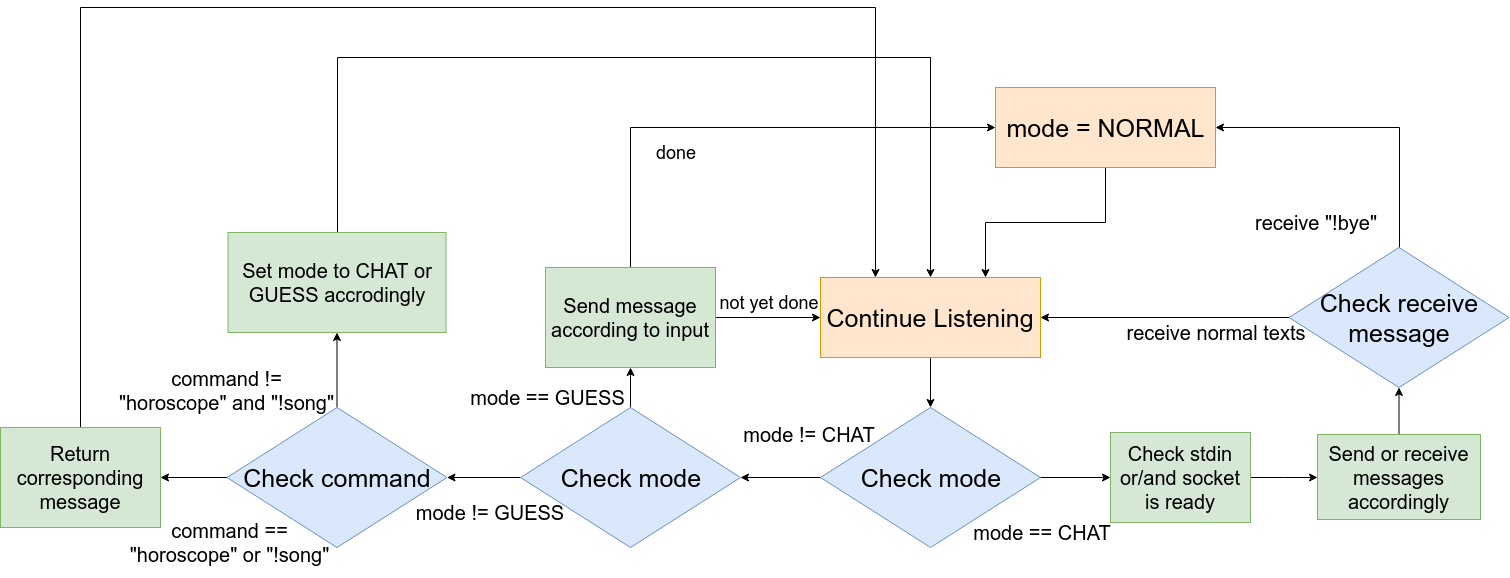
\includegraphics[width=\textwidth]{flow.png}
\end{figure}

\section{Challenges \& Solutions}

\subsection{Unable to connect to Freenode by personal hotspot}
The first I tried to connect to Freenode by Irssi, I used my personal hotspot to access the Internet, since the public wifi (NTU, ntu-peap) is unstable at my location.
However, I found that Irssi can't successfully authenticate my connection.
After several tries, I decided to change a location and use ntu-peap.
Then, everything worked as expected.

\subsection{No response}
Other client has no response to my message no matter what I sent.
After browsing on-line, I found that I forgot to add an EOL in my message.

\subsection{Cannot determine the type of commands}
I want to use "str.endswith" to detect the type of commands.
Thus, I need to remove the trailing newline characters at the end of the received messages.

\subsection{Simultaneously receiving and typing text}
To realize the "!chat" command, I use the linux "select" command via python, so that the program can simultaneously receiving and typing text.
Also, I have to print the backspace character ``\textbackslash b'' to erase the ``> '' when text was received.

\section{Reflections}
This is a very interesting assignments because it realizes the procedure of chatting online, which is heavily used nowadays after the appearance of social networks, such as Facebook, Line.
Additionally, I think it would be more interesting if students can work in group to implement a more sophisticated chatting system.

\end{document}
